\documentclass{article}

\usepackage[english]{babel}
\usepackage{amssymb, amsmath, geometry, tikz}
\geometry{top=2cm, bottom=2cm, left=3cm, right=3cm}

\title{Leader Election in Asynchronous Rings}
\author{Tsimafei Baliukonis}
\date{January 2025}

\usepackage{biblatex}
\begin{filecontents*}[overwrite]{general.bib}
@article{hirschberg1980,
  author = {D.S. Hirschberg and J.B. Sinclair},
  title = {Decentralized Extrema Finding in Circular Configurations of Processors},
  journal = {Communications of the ACM},
  year = {1980},
  volume = {23},
  number = {11},
  pages = {627--628},  
}
\end{filecontents*}
\addbibresource{general.bib}
\nocite{*}

\begin{document}

\maketitle

\section{Problem Statement}
We have an unknown number of asynchronous processors, each with a unique ID. Each processor is connected to two neighbors in a cyclic topology, forming a ring. Processors can send and receive distinguishable messages to and from their neighbors. However, a processor does not know which neighbor is to its "right" or "left" in the ring.


\begin{center}
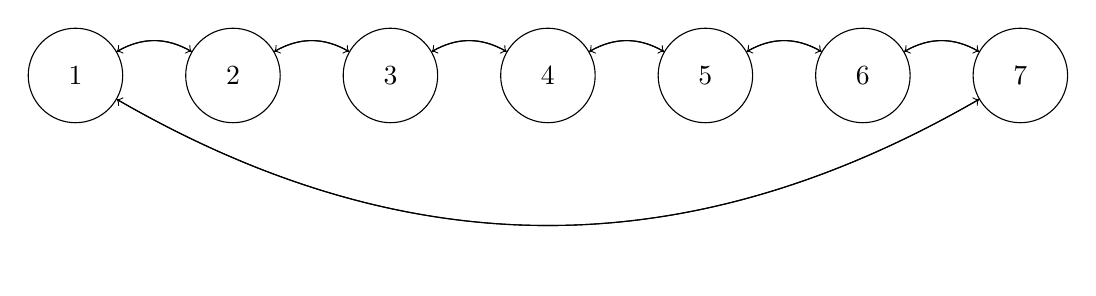
\begin{tikzpicture}[node distance=2cm, every node/.style={circle, draw, fill=white!20, minimum size=12mm}]
  \node (1) {1};
  \node (2) [right of=1] {2};
  \node (3) [right of=2] {3};
  \node (4) [right of=3] {4};
  \node (5) [right of=4] {5};
  \node (6) [right of=5] {6};
  \node (7) [right of=6] {7};

  \path[->] (1) edge[bend left] (2);
  \path[->] (2) edge[bend left] (3);
  \path[->] (3) edge[bend left] (4);
  \path[->] (4) edge[bend left] (5);
  \path[->] (5) edge[bend left] (6);
  \path[->] (6) edge[bend left] (7);
  \path[->] (7) edge[bend left] (1);

  \path[->] (2) edge[bend right] (1);
  \path[->] (3) edge[bend right] (2);
  \path[->] (4) edge[bend right] (3);
  \path[->] (5) edge[bend right] (4);
  \path[->] (6) edge[bend right] (5);
  \path[->] (7) edge[bend right] (6);
  \path[->] (1) edge[bend right] (7);
\end{tikzpicture}
\end{center}

The goal is to determine which processor has the maximum ID while minimizing the number of messages exchanged.

\section{Proposed Algorithm}
In 1980, Hirschberg and Sinclair proposed an algorithm that requires $O(n \log n)$ messages, where $n$ is the number of processors in the system.

The algorithm starts by having each processor declare itself as a candidate in the election. The process then proceeds as follows.

At stage $i$, a candidate checks whether it has the highest ID among $2^i$ neighbors in both directions. If it does, it moves to the next stage. Otherwise, it withdraws from the election. If, after $2^i$ steps in one direction, the candidate returns to itself without encountering a higher ID, it declares itself the leader.

Only the processor with the maximum ID will declare itself as the leader, while all other candidates will eventually withdraw.

\section{Message Handling}
Messages are distinguishable, allowing processors to respond to the sender or forward the message in the same direction.

At stage $i$, each processor does the following:
\begin{itemize}
  \item It checks if it is still a candidate.
  \item If true, it sends the following message to both neighbors:
  \[
    \{\text{from}, \text{process\_id}, 0, 2^i\}
  \]
  \item The processor waits for two responses:
  \begin{itemize}
    \item If it receives a message of the form \{no, process\_id\}, it withdraws.
    \item If it receives two messages of the form \{ok, process\_id\}, it proceeds to stage $i+1$.
    \item If it receives a message of the form \{from, process\_id, x, $2^i$\}, that completes a full cycle, it declares itself as the leader.
  \end{itemize}
\end{itemize}

Additionally, each processor must handle the messages it receives from other processors:
\begin{itemize}
  \item If a processor receives a message of the form \{from, sender\_id, x, y\}:
  \begin{itemize}
    \item If $\text{sender\_id} < \text{id}$, it sends back a \{no, sender\_id\} message.
    \item If $\text{sender\_id} > \text{id}$, it forwards the message further: \begin{itemize}
      \item If $x + 1 = y$, it returns an \{ok, sender\_id\} message.
      \item Otherwise, it forwards \{from, sender\_id, x + 1, y\} to the next neighbor.
    \end{itemize}
  \end{itemize}
  \item If a processor receives a message of the form \{ok, adressant\_id\} or \{no, adressant\_id\} and \text{adressant\_id} $\neq$ \text{id}, it forwards the message in the same direction.
\end{itemize}


\section{Analysis of Complexity}
At stage $i$, all remaining candidates send messages. The maximum number of participants at this stage is approximately $n / (2^i + 1)$. Each message travels a distance of up to $2^i$ in both directions and returns. Therefore, each candidate sends $2^{i+2}$ messages at stage $i$.

The total number of messages sent is bounded by:
\[ 4 \cdot \left(n + 2 \cdot \left\lfloor \frac{n}{2} \right\rfloor + 4 \cdot \left\lfloor \frac{n}{3} \right\rfloor + 8 \cdot \left\lfloor \frac{n}{5} \right\rfloor + \dots \right) \]
Since each term is not greater than $2n$, and there are at most $\log n$ terms, the total complexity is $O(n \log n)$ messages.

\printbibliography

\end{document}